\documentclass[10pt]{article}
\usepackage[usenames]{color} %used for font color
\usepackage{amssymb} %maths
\usepackage{amsmath} %maths
\usepackage[utf8]{inputenc} %useful to type directly diacritic characters
\usepackage{tikz}
\usetikzlibrary{arrows,positioning,decorations.pathreplacing} 

\definecolor{boiseBlue} {RGB}{29,72,159}
\definecolor{rojoAmor} {RGB}{171,13,4}
\definecolor{moradoAmor} {RGB}{93,8,113}
\definecolor{verdeAmor} {RGB}{98,158,31}
\definecolor{negro} {RGB}{10,10,10}
\definecolor{lgreen} {RGB}{180,210,100}
\definecolor{dblue}  {RGB}{20,66,129}
\definecolor{ddblue} {RGB}{11,36,69}
\definecolor{lred}   {RGB}{220,0,0}
\definecolor{nred}   {RGB}{224,0,0}
\definecolor{norange}{RGB}{230,120,20}
\definecolor{nyellow}{RGB}{255,221,0}
\definecolor{ngreen} {RGB}{98,158,31}
\definecolor{dgreen} {RGB}{78,138,21}
\definecolor{nblue}  {RGB}{28,130,185}
\definecolor{jblue}  {RGB}{20,50,100}\begin{document}
\[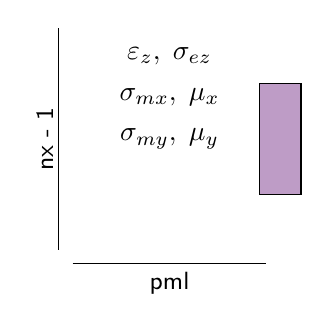
\begin{tikzpicture}
%
%\node[draw=black,fill=nyellow!40,minimum width=7em,minimum height=8em,rectangle]  at (0,0) {};
 \node[draw=black,fill=moradoAmor!40,minimum width=1.5em,minimum height=4em,rectangle]  at (4em,0em) {}; % 2.25em
%
\node[]  at (0em,3em) {$\varepsilon_{z}, \; \sigma_{ez}$};
\node[]  at (0em,1.5em) {$\sigma_{mx}, \; \mu_{x}$};
\node[]  at (0em,0em) {$\sigma_{my}, \; \mu_{y}$};
%\node[]  at (0,-1.5em) {$\mu_{x}$};
%
%\draw[] (-4em,3em) -- (-4em,4em);
\draw[] (-4em,-4em) -- (-4em,4em);
% \node[rotate=90]  at (-4.5em,3.5em) {\small{\sf 2}};
\node[rotate=90]  at (-4.5em,0) {\small{\sf nx - 1}};
% \draw[] (-6em,1.5em) -- (-6em,4em);
% \draw[] (-6em,-2em) -- (-6em,4em);
% \node[rotate=90]  at (-6.5em,2.5em) {\small{\sf pis}};
% \node[rotate=90]  at (-6.5em,1em) {\small{\sf nx}};
\draw[] (-3.5em,-4.5em) -- (3.5em,-4.5em);
\node[]  at (0,-5.2em) {\small{\sf pml}};
% \draw[] (-3.5em,-6em) -- (2.75em,-6em);
% \node[]  at (0em,-6.8em) {\small{\sf ny}};
%
\end{tikzpicture}
\]
\end{document}